\documentclass[tikz]{standalone}

\usepackage{tikz}
\usetikzlibrary{trees}
\usetikzlibrary{shapes}
\usetikzlibrary{positioning}
\usetikzlibrary{arrows.meta}

\tikzset{
    mynode/.style = {circle, ultra thick, draw=black, align=center,fill=yellow!30,font=\ttfamily\bfseries\Large,text=black},
    mynoder/.style = {circle, ultra thick, draw=black, align=center,fill=red!30,font=\ttfamily\bfseries\Large,text=black},
    mynodeb/.style = {circle, ultra thick, draw=black, align=center,fill=blue!30,font=\ttfamily\bfseries\Large,text=black},
    mynodeg/.style = {circle, ultra thick, draw=gray, align=center,fill=gray!05,font=\ttfamily\bfseries\Large,text=gray!20},
    mynodegr/.style = {circle, ultra thick, draw=gray, align=center,fill=gray!05,font=\ttfamily\bfseries\Large,text=red},
    edgen/.style = {-,ultra thick,black},
    edger/.style = {-,ultra thick,red},
    edgeb/.style = {-,ultra thick,blue},
    edgeg/.style = {-,ultra thick,gray},
    edgegd/.style = {-,ultra thick,brown,dashed}, % back
    edgevd/.style = {-,ultra thick,violet,dotted}, % forward
    edgexd/.style = {-,ultra thick,blue,densely dotted}, % traversal
    every picture/.style={/utils/exec={\ttfamily\bfseries}},
    every picture/.style={font issue=\ttfamily\bfseries},
    font issue/.style={execute at begin picture={#1\selectfont}}
}

\begin{document}

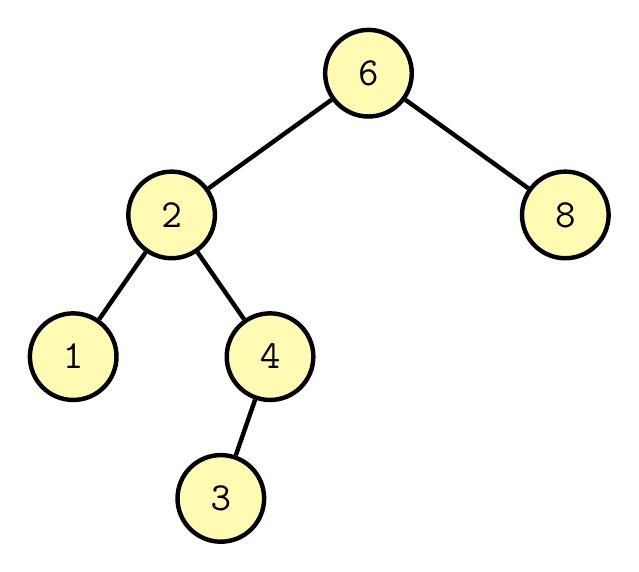
\begin{tikzpicture}[
	level distance=1.8cm,
    level 1/.style={sibling distance=5cm},
    level 2/.style={sibling distance=2.5cm},
    level 3/.style={sibling distance=1.25cm},
	thick,
    minimum width={1.1cm},
	font=\ttfamily\bfseries]
    
  \node[mynode] {6}
    child [edgen] {node[mynode] {2}
      child [edgen] {node[mynode] {1}}
      child [edgen] {node[mynode] {4}
        child [edgen] {node[mynode] {3}}
        child[missing] {node[mynode] {}}
      }
    }
    child [edgen] {node[mynode] {8}}
    ;

\end{tikzpicture}

\newpage

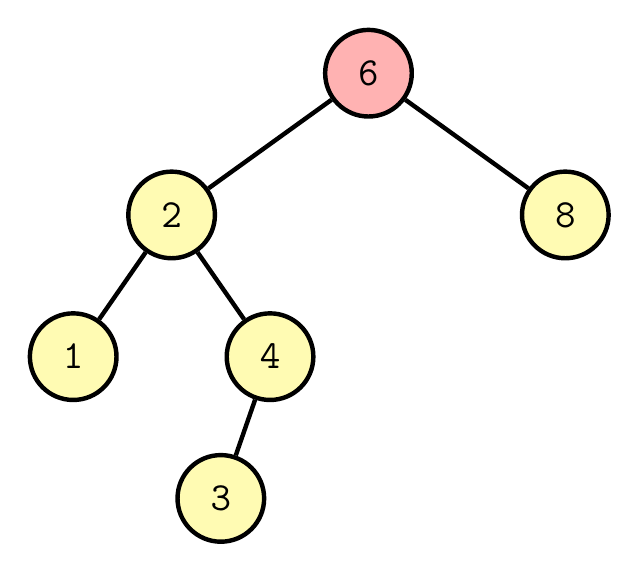
\begin{tikzpicture}[
	level distance=1.8cm,
    level 1/.style={sibling distance=5cm},
    level 2/.style={sibling distance=2.5cm},
    level 3/.style={sibling distance=1.25cm},
	thick,
    minimum width={1.1cm},
	font=\ttfamily\bfseries]
    
  \node[mynoder] {6}
    child[edgen] {node[mynode] {2}
      child[edgen] {node[mynode] {1}}
      child[edgen] {node[mynode] {4}
        child[edgen] {node[mynode] {3}}
        child[missing] {node[mynode] {}}
      }
    }
    child[edgen] {node[mynode] {8}}
    ;

\end{tikzpicture}

\newpage

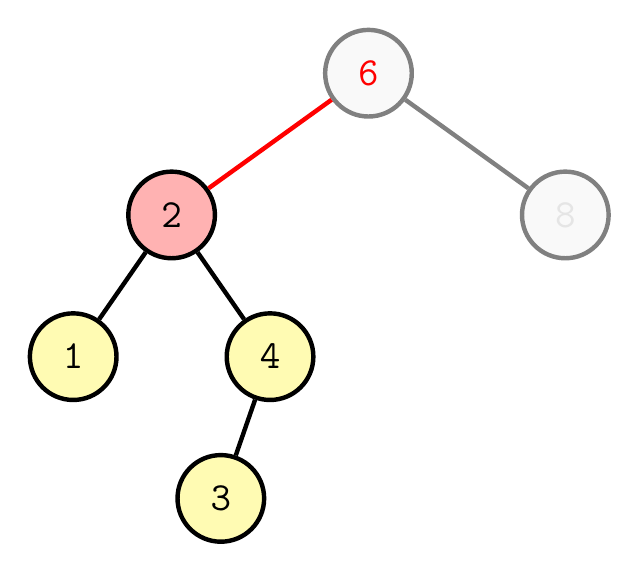
\begin{tikzpicture}[
	level distance=1.8cm,
    level 1/.style={sibling distance=5cm},
    level 2/.style={sibling distance=2.5cm},
    level 3/.style={sibling distance=1.25cm},
	thick,
    minimum width={1.1cm},
	font=\ttfamily\bfseries]
    
  \node[mynodeg,text=red] {6}
    child[edger] {node[mynoder] {2}
      child[edgen] {node[mynode] {1}}
      child[edgen] {node[mynode] {4}
        child[edgen] {node[mynode] {3}}
        child[missing] {node[mynode] {}}
      }
    }
    child[edgeg] {node[mynodeg] {8}}
    ;

\end{tikzpicture}

\newpage

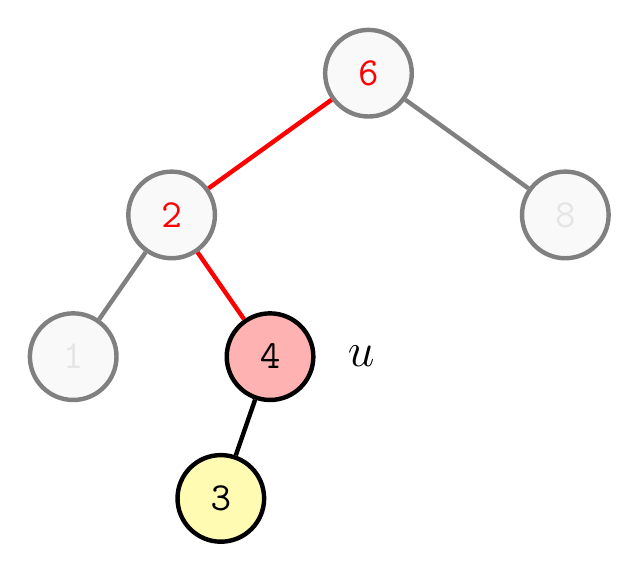
\begin{tikzpicture}[
	level distance=1.8cm,
    level 1/.style={sibling distance=5cm},
    level 2/.style={sibling distance=2.5cm},
    level 3/.style={sibling distance=1.25cm},
	thick,
    minimum width={1.1cm},
	font=\ttfamily\bfseries]
    
  \node[mynodeg,text=red] {6}
    child[edger] {node[mynodeg,text=red] {2}
      child[edgeg] {node[mynodeg] {1}}
      child[edger] {node[mynoder, label={right:\LARGE \textcolor{black}{$u$}}] {4}
        child[edgen] {node[mynode] {3}}
        child[missing] {node[mynode] {}}
      }
    }
    child[edgeg] {node[mynodeg] {8}}
    ;

\end{tikzpicture}


\newpage

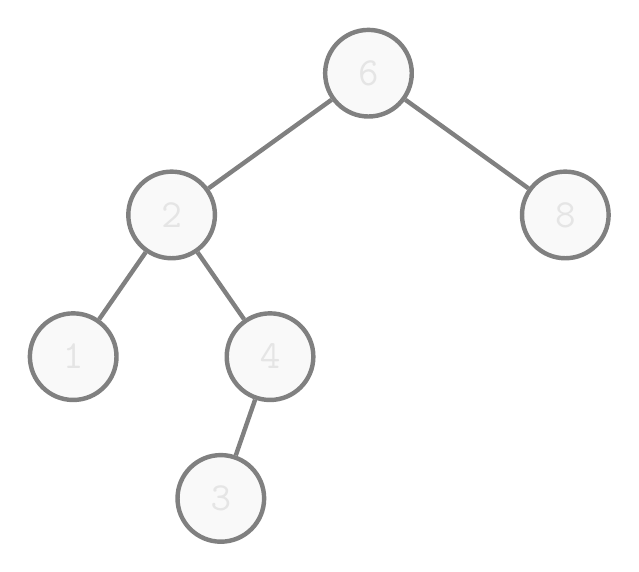
\begin{tikzpicture}[
	level distance=1.8cm,
    level 1/.style={sibling distance=5cm},
    level 2/.style={sibling distance=2.5cm},
    level 3/.style={sibling distance=1.25cm},
	thick,
    minimum width={1.1cm},
	font=\ttfamily\bfseries]
    
  \node[mynodeg] {6}
    child[edgeg] {node[mynodeg] {2}
      child[edgeg] {node[mynodeg] {1}}
      child[edgeg] {node[mynodeg] {4}
        child[edgeg] {node[mynodeg] {3}}
        child[missing] {node[mynode] {}}
      }
    }
    child[edgeg] {node[mynodeg] {8}}
    ;

\end{tikzpicture}


\end{document}